\documentclass{hfutpaper}
\usepackage[urlcolor=blue]{hyperref}
\usepackage{threeparttable}
\usepackage{setspace}
\usepackage{titlesec}
\usepackage{verbatim}
\usepackage{listings}
\usepackage{float}
\newcommand{\upcite}[1]{\textsuperscript{\textsuperscript{\cite{#1}}}}
\usepackage{fancyhdr}
\titleformat{\section}{\large \heiti}{\chinese{section}、}{0em}{}
\begin{document}
\begin{center}
\LARGE
  \textbf{MIPS单周期CPU设计\ 实验报告}\\
  \vspace{0.2em}
  \large
    程宇笑\ 自84 2018010888
  \end{center}
  

\section{数据通路结构设计}

\par 根据所学知识设计简单集指令单周期MIPS数据通路。为了简化设计流程,在仿真设计工程中暂不加入涉及外设硬件的输入输出模块,同时使用Verilog描述的寄存器堆和多路选择器模拟的RAM和ROM。总体数据通路电路如下:

% 图片
\begin{figure}[H]
	\centering
	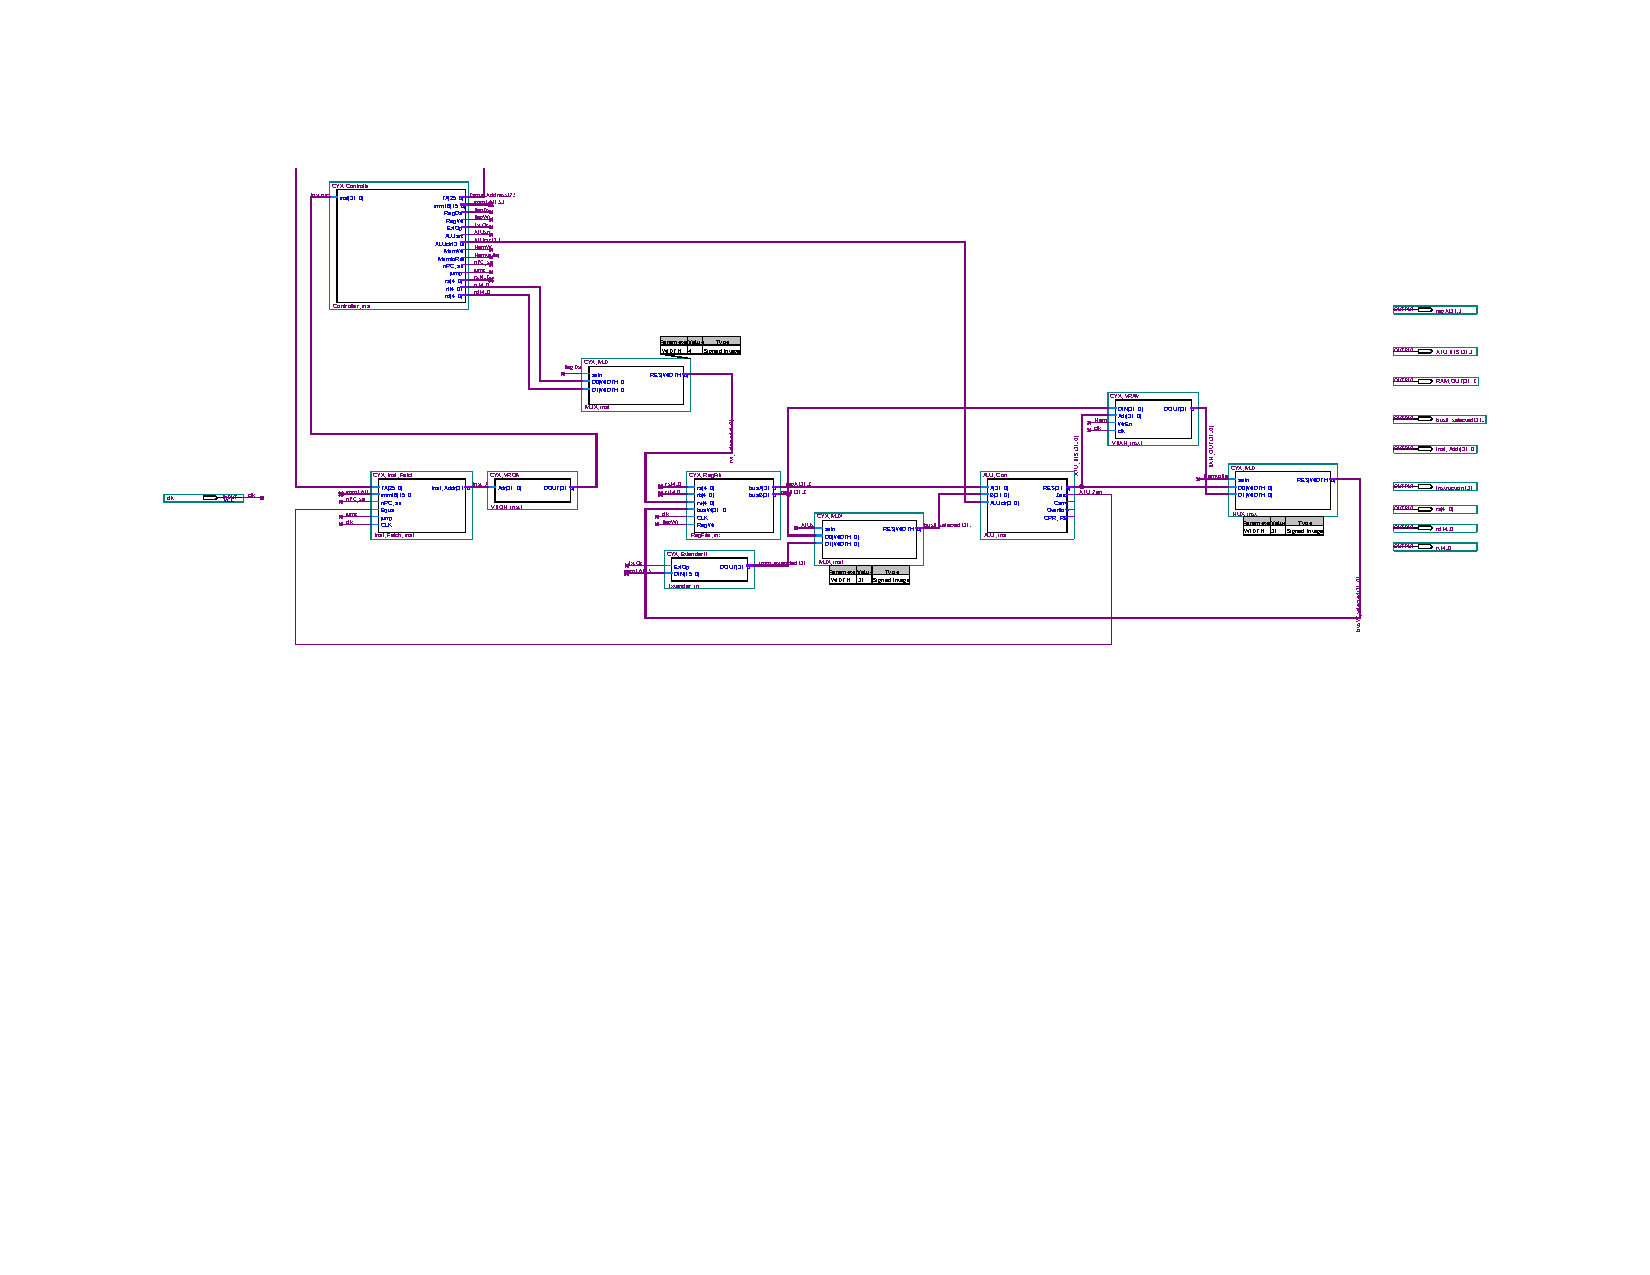
\includegraphics[width = \textwidth]{bdf}
\end{figure}

\par 该电路总共使用9个通过Verilog描述的模块。

\subsection{各模块设计}

\par 该单周期CPU的9个模块分别为ALU核心、寄存器堆、取指令模块、控制器、多选器、立即数扩展器、虚拟RAM、虚拟ROM。
\par \textbf{ALU核心(ALU\_Core):}使用实验二设计的ALU模块,但需要将比较结果输出端口与主输出端口合并,即设置为比较功能时如果A与B相等则输出32位的0。
\par \textbf{寄存器堆(RegFile):}含有8个32位寄存器,使用Verilog描述其初始化和读写功能。

\begin{lstlisting}[language=verilog]
	assign busA = regs[ra];
	assign busB = regs[rb];
	
	always @ (posedge CLK) begin
		regs[0] = REG0_DATA;
		if (RegWr && (rw != 0)) begin
			regs[rw] = busW;
		end
	end
\end{lstlisting}

\par \textbf{取指令模块(Inst\_Fetch):}支持顺序执行、PC相对寻址(beq指令)和伪直接寻址(j指令)。除此之外,还包含立即数扩展功能(符号位扩展14位,结尾加两个0)和PC寄存器,计算指令地址完成后传给虚拟ROM。
\par \textbf{虚拟ROM(VROM):}为了方便调试和开发,直接使用Verilog描述ROM内含数据,通过类似于多选器的描述方式实现ROM功能。读取到指令内容后交给控制器。

\begin{lstlisting}[language=verilog]
	case (Adr)
			
		0: DOUT = 32'h8c220000; //lw $2, 0($1)
		4: DOUT = 32'h8c230004; //lw $3, 4($1)
		8: DOUT = 32'h8c240008; //main: lw $4, 8($1)
		...
		default:	DOUT = 32'h0;
	endcase
\end{lstlisting}

\par \textbf{控制器(Controller):}读取指令内容,解析出各字段含义及控制信号。该模块本质上是组合逻辑电路模块。
\par \textbf{多选器(MUX):}用于控制信号对数据的选择。
\par \textbf{立即数扩展器(Extender16):}用于立即数的输入,分为0扩展和符号扩展两种模式。
\par \textbf{虚拟RAM(VRAM):}使用Verilog描述,其行为与寄存器堆类似。可以在任意时刻读取数据,在时钟上升沿写入数据。

\section{仿真分析}

\par 使用如下的MIPS汇编程序进行测试,其本身是一个循环。在内存的0,4,8地址中预先填充数据1,2,-1。设置输出信号,然后进行时序仿真。


\begin{lstlisting}[language=python]
		lw $2, 0($1)
		lw $3, 4($1)
	main:
		lw $4, 8($1)
		add $6, $2, $6
		sub $5, $3, $4
		sw $5, 8($1)
		or $5, $4, $3
		and $5, $4, $3
		slt $5, $6, $3
		beq $6, $3, exit
		j main
	exit:	lw $2, 0($3)
		j main
\end{lstlisting}

\subsection{数据通路时序分析}

\par 截取单个时钟上升沿之后的波形图进行观察,可以发现信号发生改变的时间顺序可以列举如下。该时序符合理论设计。

\begin{itemize}
	\item 取指令模块:PC寄存器的输出(Inst\_Addr)
	\item 虚拟ROM:指令内容(Instruction)
	\item 控制器:rs、rt、rd等信号
	\item 寄存器堆:regA等读取出的数据
	\item ALU核心:运算结果(ALU\_RES)
	\item 虚拟RAM:内存读取结果(RAM\_OUT)
\end{itemize} 
% 图片
\begin{figure}[H]
	\centering
	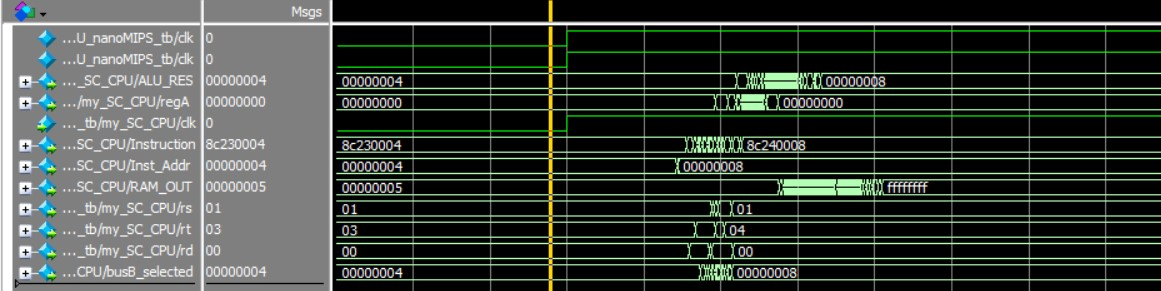
\includegraphics[width = \textwidth]{timing}
\end{figure}

\subsection{程序执行逻辑分析}

\par 程序先从内存中读取数据1、5、-1到寄存器2、3、4,然后开始循环。每次循环给寄存器6累加1,直到寄存器6的值等于寄存器3的值(即5),跳转到exit标签。程序执行的波形图符合预期:
% 图片
\begin{figure}[H]
	\centering
	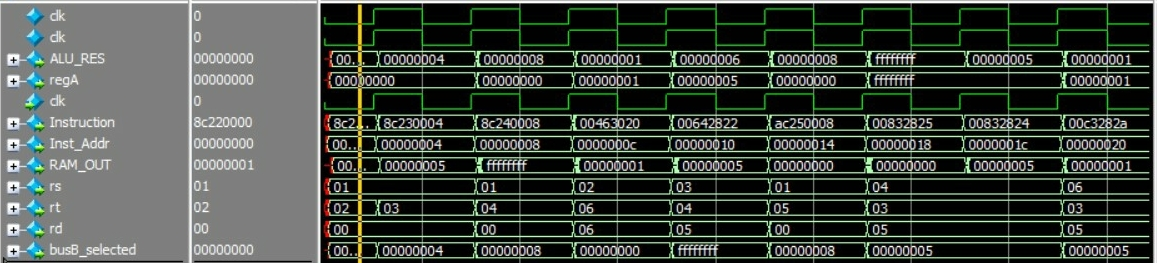
\includegraphics[width = \textwidth]{timing1}
\end{figure}
% 图片
\begin{figure}[H]
	\centering
	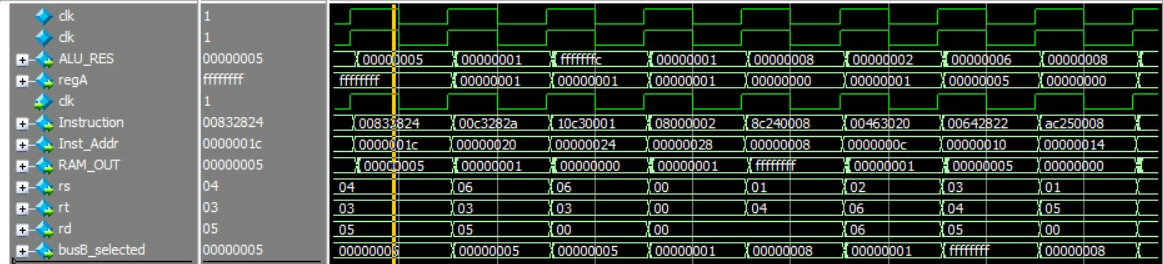
\includegraphics[width = \textwidth]{timing2}
\end{figure}


\section{硬件实验和signalTap II分析}

\par 为了便于观察,设置时钟周期为1Hz。加入数码管扫描模块并设置输入输出端口后烧录进FPGA,硬件测试电路如图(可以通过发光二极管观察时钟信号、ALUsrc、RegWr、RegDst信号,通过数码管可以观察ALU计算结果的最后四位)。

% 图片
\begin{figure}[H]
	\centering
	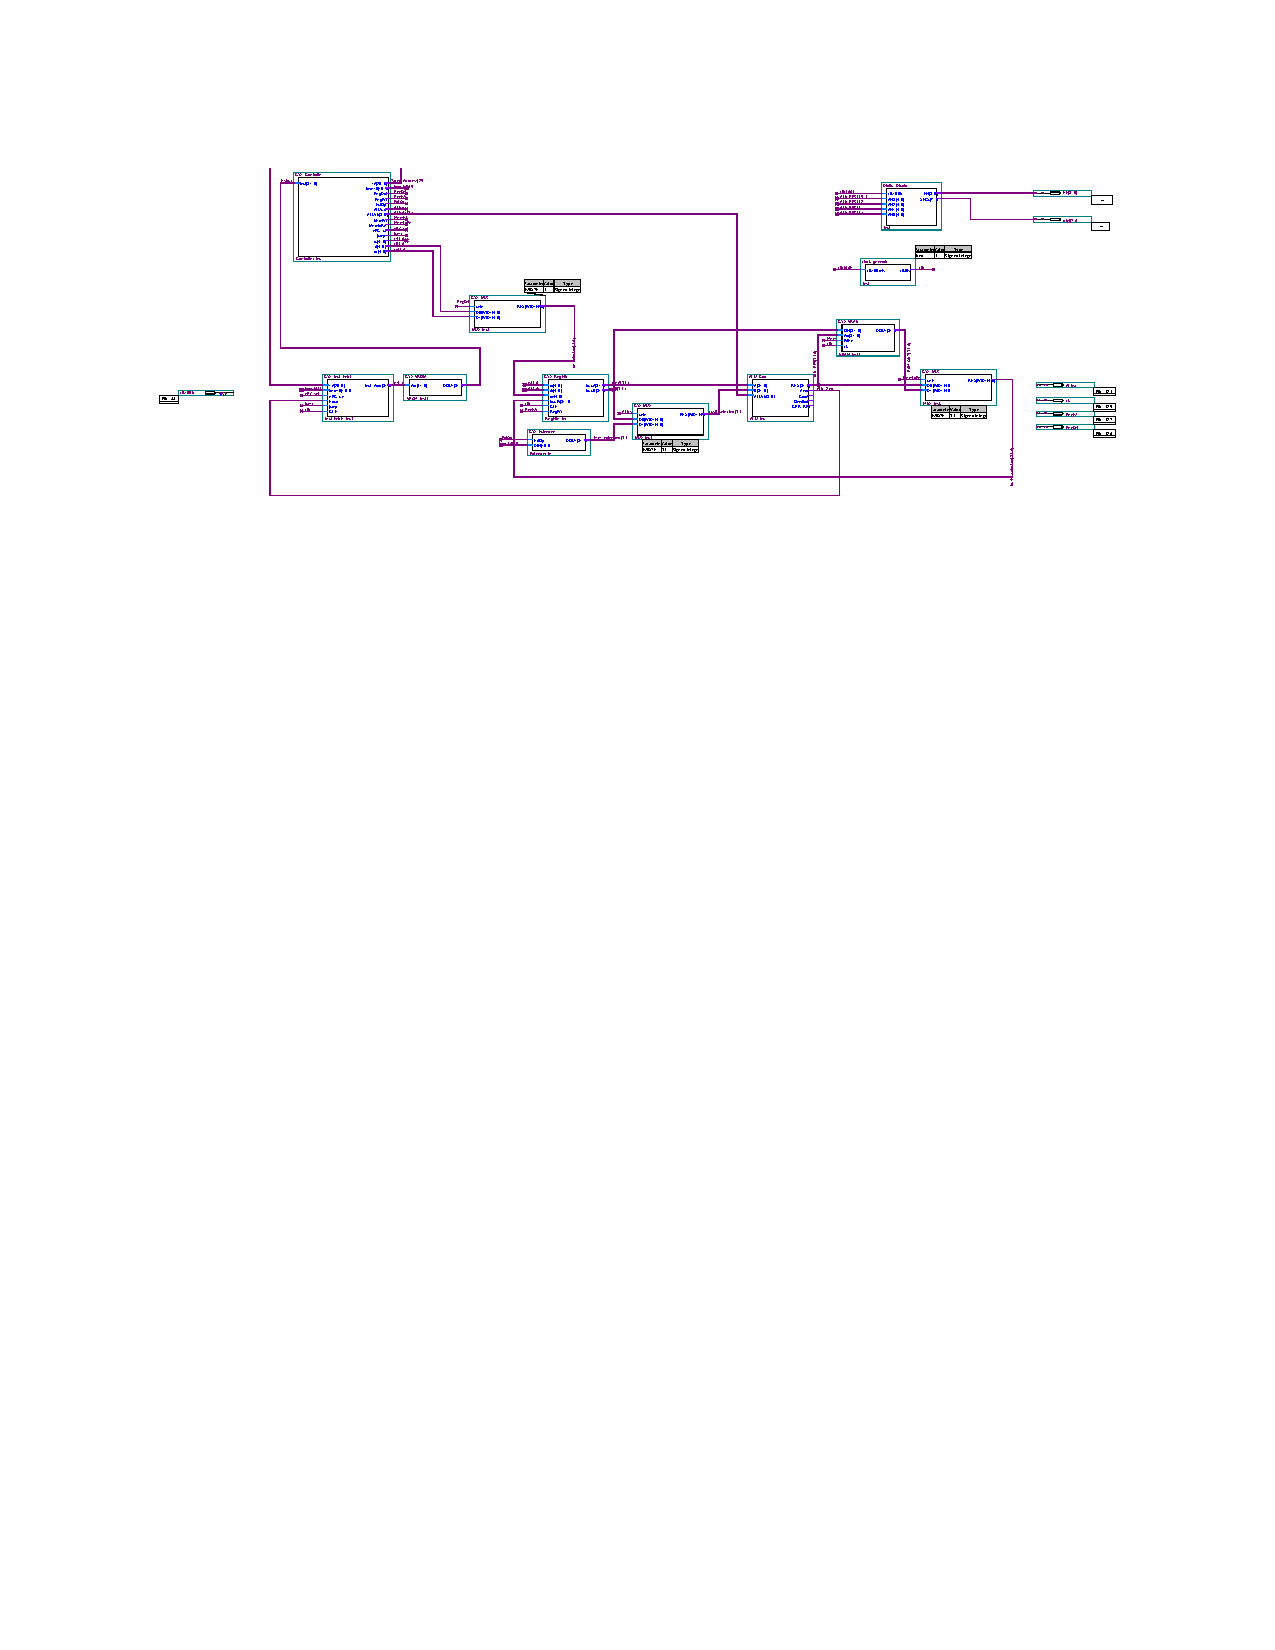
\includegraphics[width = \textwidth]{hardware}
	\caption{加入输入输出模块的硬件实验电路}
\end{figure}

\par 经过观察发现,通过LED和数码管现实的各信号值的时间顺序符合预期。
% 图片
\begin{figure}[H]
	\centering
	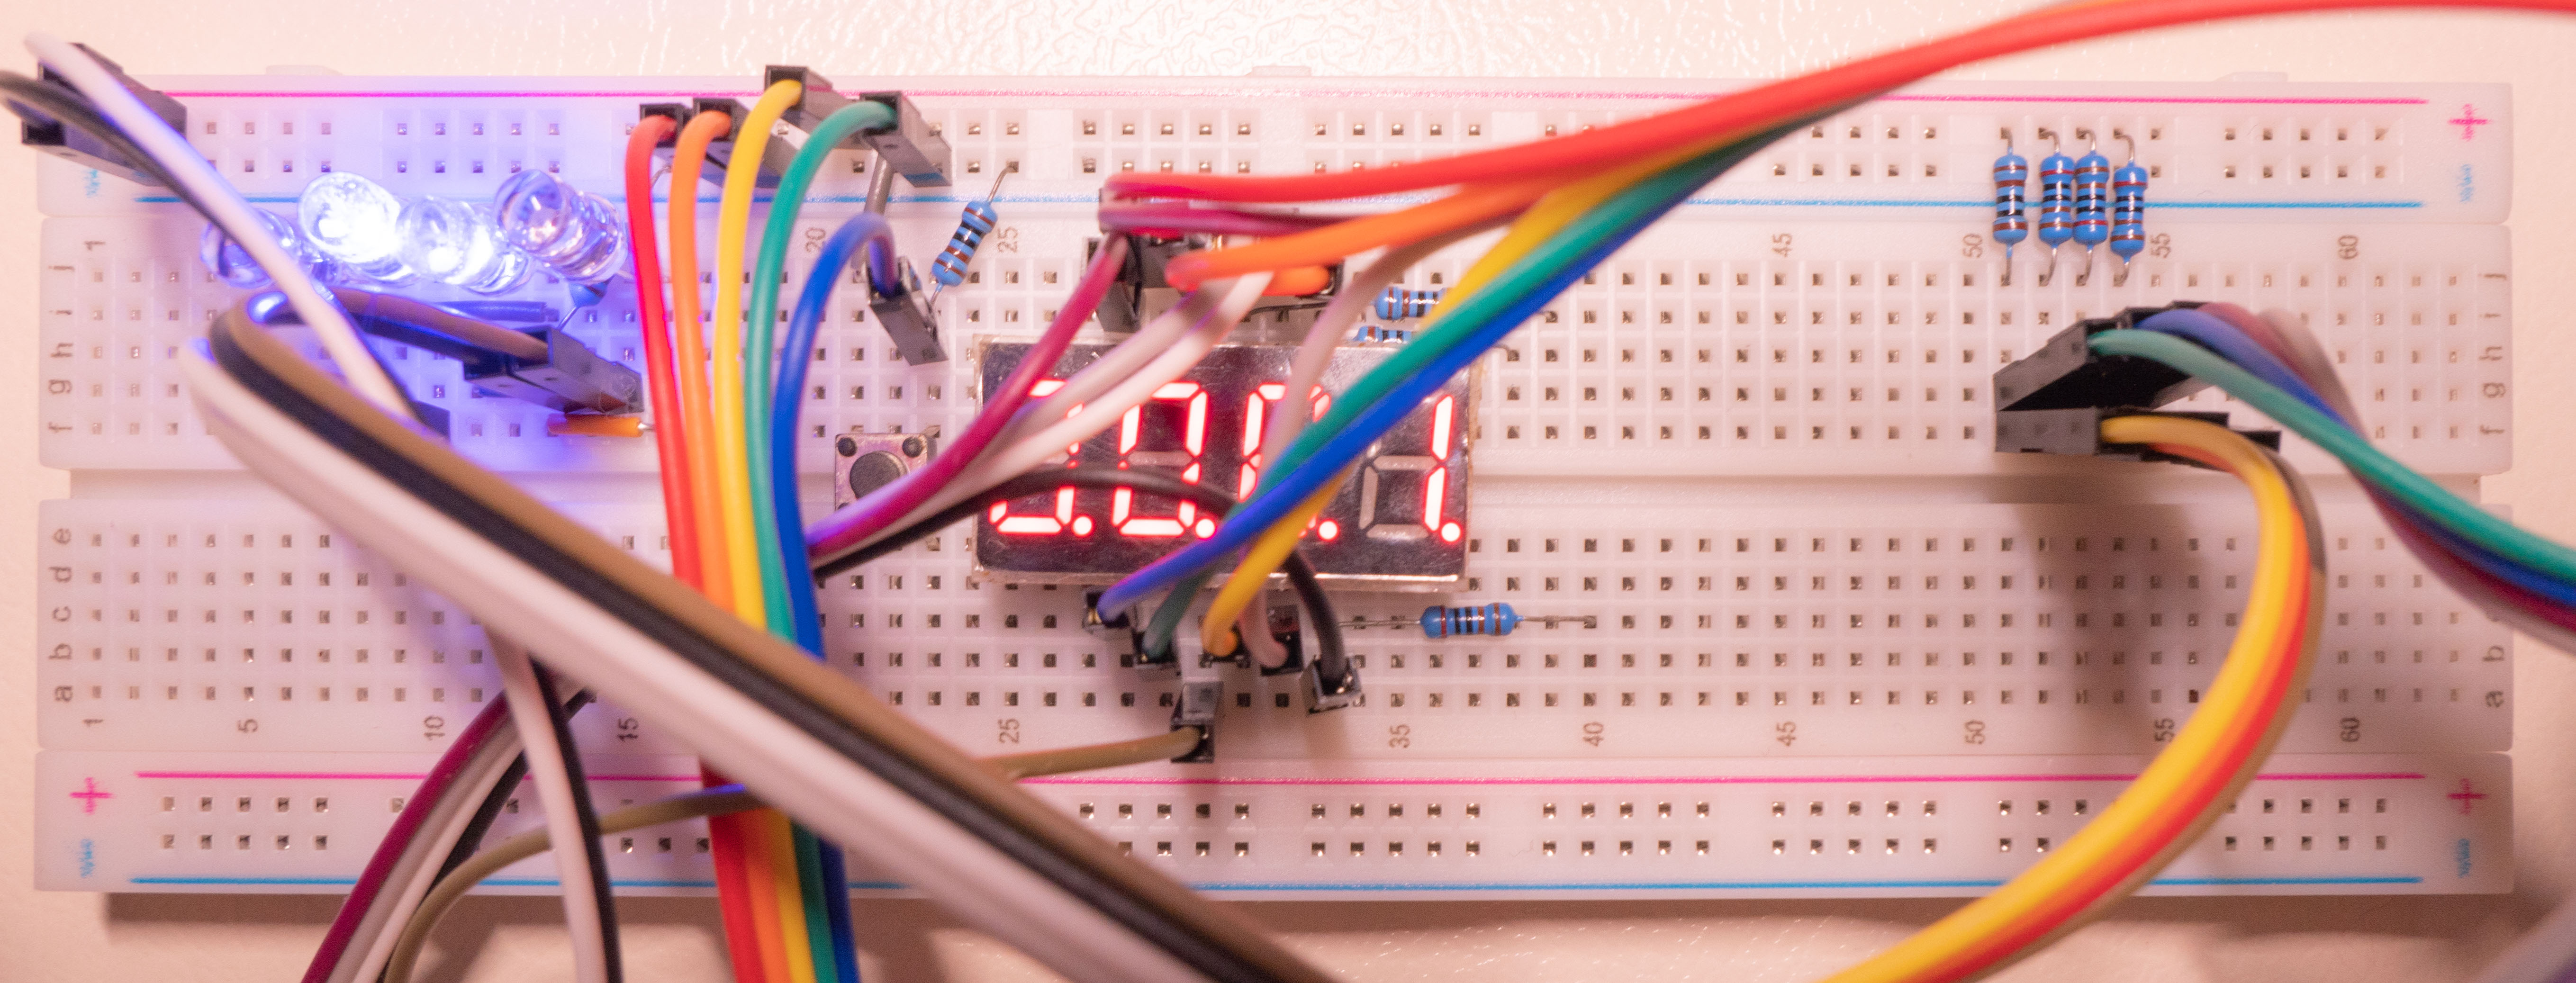
\includegraphics[width = \textwidth]{breadboard.jpg}
	\caption{面包板上搭建的外围电路}
\end{figure}

\par 设置时钟频率为10MHz后,通过signalTap II观察内部波形,结果如下,符合预期:

% 图片
\begin{figure}[H]
	\centering
	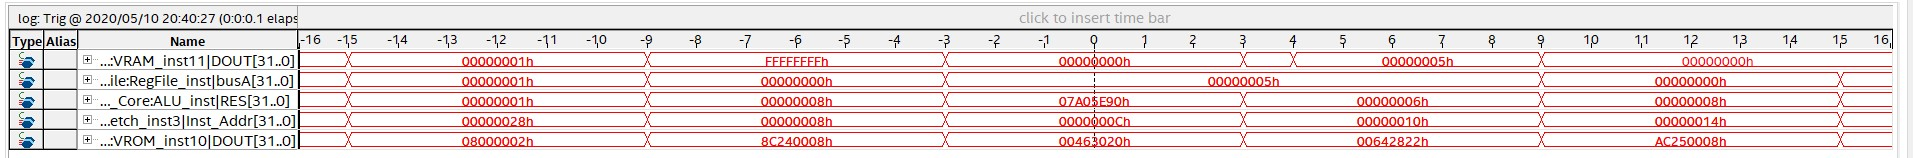
\includegraphics[width = \textwidth]{st1.jpg}
\end{figure}
% 图片
\begin{figure}[H]
	\centering
	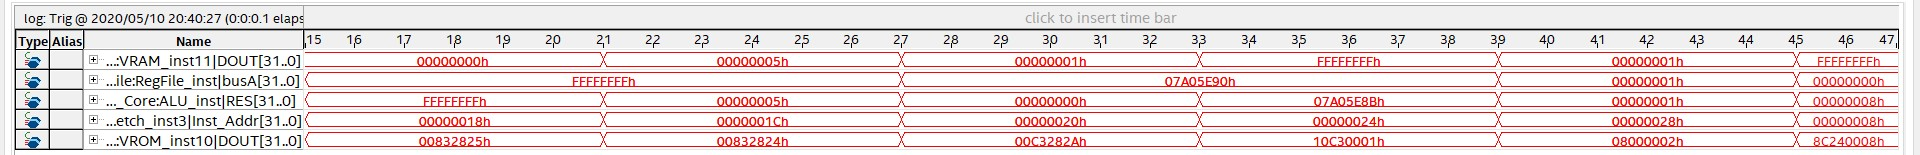
\includegraphics[width = \textwidth]{st2.jpg}
\end{figure}


\section{总结与思考}

\par 单周期CPU的设计过程中,存储器的时钟设计最让人困扰。之所以寄存器堆和主存需要在时钟沿存储数据,却不造成类似于流水线的冒险现象,是因为寄存器堆和主存(RAM)的写入操作总是在指令执行流程的最后。即便需要等待下一个时钟上升沿的到达才能写入数据,也并不影响下一个时钟周期的取指令等操作。

\par 然而如果使用Quartus软件提供的ROM宏器件(该器件具有无法去掉的读取时钟)用于存储程序,情况便有所不同。如果指令地址准备好后需要等待下一个时钟周期才能读取指令内容,那么便难以控制单周期CPU数据通路的良好运行。此时可以给ROM使用更高频率的时钟、使用相同频率但上升沿延后的时钟或者使用时钟信号的反相,从而解决该问题。

\par 在我的解决方案中,直接通过Verilog描述虚拟的RAM和ROM,规避了上述时钟混乱的问题。



\begin{comment}

% 列表
\begin{itemize}
	\item 必做任务1:三角波,频率100\ Hz,电压0$\thicksim 5\ $V.
\end{itemize} 

% 表格
\begin{table}[H]
	\begin{tabular}{l|llllllllllll}
	\hline
	$R_1 / \Omega$ & 0k    & 0.5k & 1k   & 2k    & 3k    & 4k    & 5k   & 6k    & 7k    & 8k    & 9k    & 10k   \\ \hline
	$I_{p-p} / mA$ & 0.042 & 1.34 & 1    & 0.64 & 0.45 & 0.35 & 0.29 & 0.24 & 0.21  & 0.18 & 0.17 & 0.15  \\ \hline
	$I_{rms} / mA$ & 0.015 & 0.47 & 0.35 & 0.22  & 0.16  & 0.12  & 0.10 & 0.086 & 0.074 & 0.065 & 0.058 & 0.053 \\ \hline
	\end{tabular}
\end{table}

% 图片
\begin{figure}[H]
	\centering
	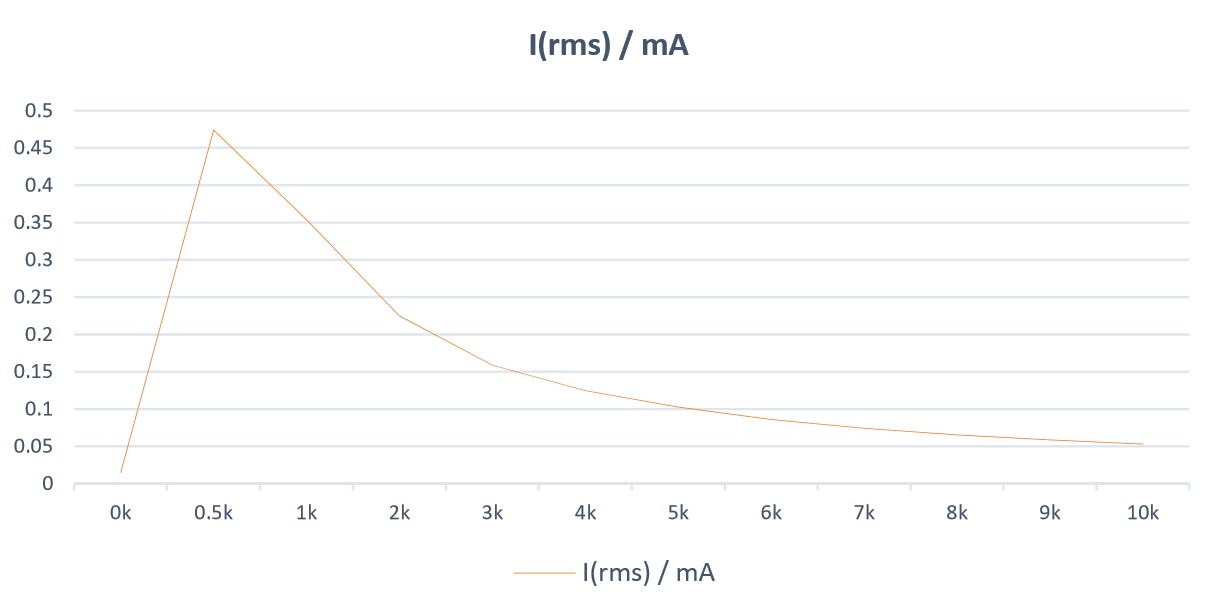
\includegraphics[width = 0.8\textwidth]{1}
\end{figure}

% 双图
\begin{figure}[htb]	
	\begin{minipage}[b]{0.5\textwidth} 
	  \centering 
	  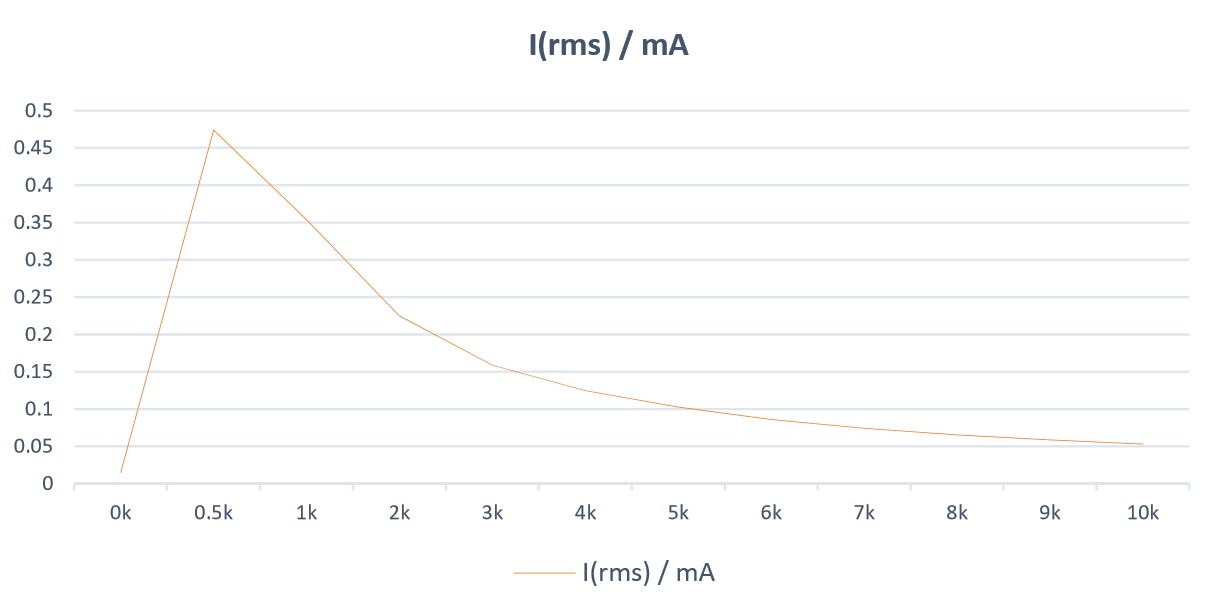
\includegraphics[width=\textwidth]{1} 
	\end{minipage}% 
	\begin{minipage}[b]{0.5\textwidth} 
	  \centering 
	  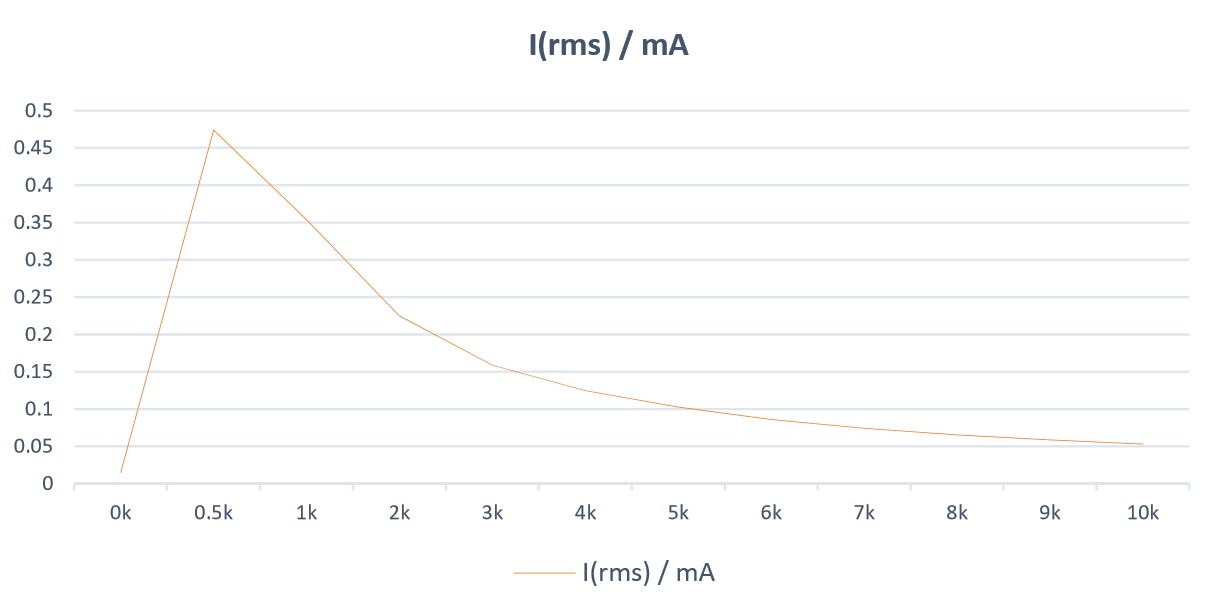
\includegraphics[width=\textwidth]{1} 
	\end{minipage}% 
	\caption{}
\end{figure}

% 图表混合
\begin{figure}[htb]	
	\begin{minipage}[b]{0.5\textwidth} 
	\centering
	\begin{tabular}{cc|cc}
		\hline
		A & B & $Y_{h}$ & $C_{Oh}$ \\  \hline
		0 & 0 & 0 & 0 \\ 
		0 & 1 & 1 & 0 \\ 
		1 & 0 & 1 & 0 \\ 
		1 & 1 & 0 & 1 \\ \hline
		\end{tabular}
	\caption{} 
	\label{table:by:fig} 
  \end{minipage}  
	\begin{minipage}[b]{0.5\textwidth} 
	  \centering 
	  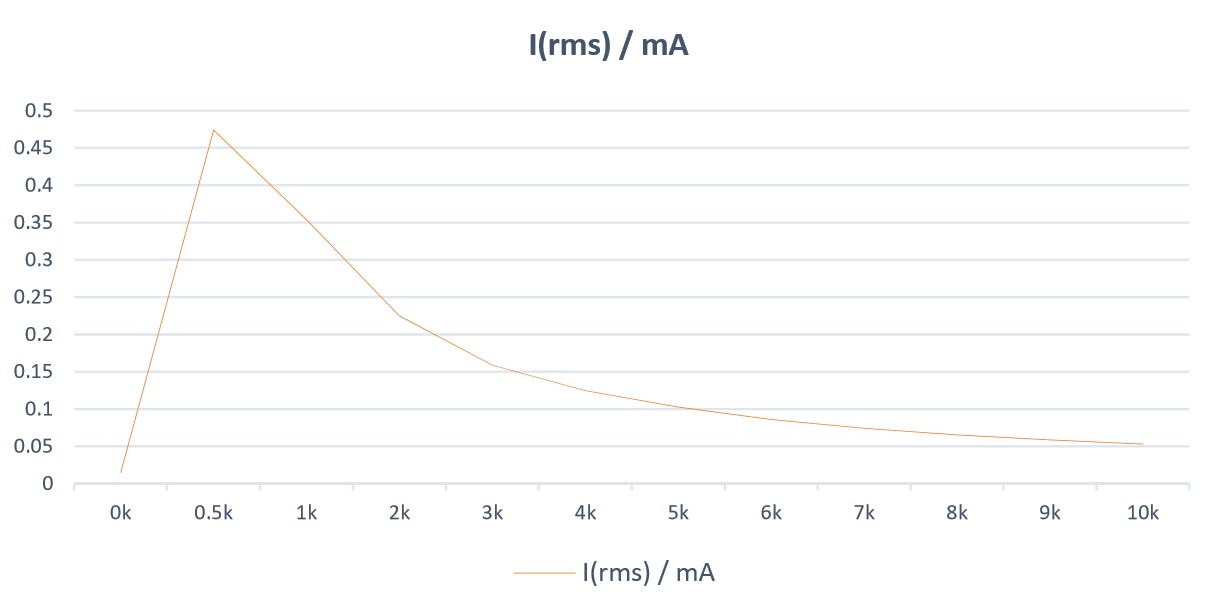
\includegraphics[width=0.7\textwidth]{1} 
	  \caption{} 
	  \label{fig:by:table} 
	\end{minipage}% 
\end{figure}

\begin{lstlisting}[language=c++]
#include <iostream>
int main()
{
    std::cout << "Hello, World!" << std::endl;
}  
\end{lstlisting}

\end{comment}

\end{document} 